\documentclass{article}
\usepackage{amsmath}
\usepackage{amssymb}
\usepackage{indentfirst}
\usepackage{color}
\usepackage{graphicx}
\usepackage{epstopdf}
\usepackage{geometry}
\geometry{left=2.5cm,right=2.5cm,top=2.5cm,bottom=2.5cm}

\title{14.03 Problem Set 2}
\author{Yijun Jiang}
%\email{yjjiang@mit.edu}
\date{\today}

\begin{document}
\maketitle

\section{Short Questions}
\subsection{Question 1}
\noindent\underline{Conclusion}: This statement is FALSE.

\noindent\underline{Explanation}: Brian cannot treat all goods to be inferior. An inferior good is demanded less when income increases. If all goods are inferior for Brian, when his income increases, he consumes everything less. Therefore, he cannot spend all of his budget. This violates non-satiation axiom. Brian must have at least one normal good on which he spends more than before.

\subsection{Question 2}
\noindent\underline{Conclusion}: This statement is FALSE.

\noindent\underline{Explanation}: We cannot compare utility between two individuals. This is because utility function is defined up to a monotonic transformation. It makes no sense to compare the pure value of Peter's utility with John's. Even if Peter's is larger, it does not mean anything.

\subsection{Question 3}
\noindent\underline{Conclusion}: This statement is TRUE.

\noindent\underline{Explanation}: An inferior good has negative substitution effect and negative income effect. These two effects counteract. For an ordinary inferior good, substitution effect dominates over income effect, so an increase in price leads to a decrease in consumption. A Giffen good, on the other hand, is a strongly inferior good. Its income effect dominates over substitution effect, so an increase in price leads to an increase in comsumption.

According to this definition, a Giffen good is a special type of inferior good. But a general inferior good does not necessarily need to be a Giffen good, and it is often not.

\subsection{Question 4}
\noindent\underline{Conclusion}: This statement is TRUE.

\noindent\underline{Explanation}: For an indifference curve $U(x_1,x_2,\cdots,x_n)=U_0$, the slope in $x_1$-$x_2$ plane is given by
\begin{equation*}
	\left(\frac{\partial x_1}{\partial x_2}\right)_{x_3,\cdots,x_n}=-\frac{\partial U/\partial x_2}{\partial U/\partial x_1}
\end{equation*}
where the subscipts denote the variables that are held fixed in the partial derivative. Since $U(x_1,x_2,\cdots,x_n)$ is increasing for all $x_i$ ($i=1,2,\cdots,n$), $\partial U/\partial x_i>0$. Therefore, $(\partial x_1/\partial x_2)_{x_3,\cdots,x_n}<0$, which means that the indifference curve is downward sloping in $x_1$-$x_2$ plane. The same is true for every other pair of goods.

Moreover, marginal rate of substitution of $x_1$ for $x_2$ is
\begin{equation*}
	MRS_{x_1,x_2}=-\left(\frac{\partial x_2}{\partial x_1}\right)_{x_3,\cdots,x_n}
\end{equation*}
which decreases with $x_1$ due to the property of deminishing MRS. This means
\begin{equation*}
	\left(\frac{\partial^2x_2}{\partial x_1^2}\right)_{x_3,\cdots,x_n}>0
\end{equation*}
Similarly $\left(\frac{\partial^2x_1}{\partial x_2^2}\right)_{x_3,\cdots,x_n}>0$. Therefore, the indifference curve is bowed towards the origin. The same is true for every other pair of goods.

\subsection{Question 5}
\noindent\underline{Conclusion}: This statement is FALSE.

\noindent\underline{Explanation}: The relation $MRS_{x,y}=-dy/dx=p_x/p_y$ only holds for an interior solution. When the solution is binded by the non-negative constraint, i.e. $x\geqslant0$ and $y\geqslant0$, one of the goods has zero quantity. In this case, the bundle is still maximal (under non-negative constraint), though the relation $MRS_{x,y}=p_x/p_y$ no longer holds.

\section{Utility Maximization and Marshallian Demand Functions}
\subsection{Part 1}
The utility maximization problem under budget constraint is
\begin{align*}
	&U^*=\max_{x,y}\left(\frac{1}{4}\log x+\frac{3}{4}\log y\right)\\
	&\textup{s.t. }p_xx+p_yy\leqslant m
\end{align*}

And according to non-satiation axiom, this can be rewritten as
\begin{align*}
	&U^*=\max_{x,y}\left(\frac{1}{4}\log x+\frac{3}{4}\log y\right)\\
	&\textup{s.t. }p_xx+p_yy=m
\end{align*}

We can use Lagrange multiplier $\lambda$. The problem becomes
\begin{align*}
	L(x,y,\lambda)&=\frac{1}{4}\log x+\frac{3}{4}\log y+\lambda(m-p_xx-p_yy)\\
	\frac{\partial L}{\partial x}&=0\\
	\frac{\partial L}{\partial y}&=0\\
	\frac{\partial L}{\partial\lambda}&=0
\end{align*}

This leads to
\begin{align*}
	\frac{1}{4x}-\lambda p_x&=0\\
	\frac{3}{4y}-\lambda p_y&=0\\
	p_xx+p_yy&=m
\end{align*}

The solution is
\begin{align*}
	\lambda&=\frac{1}{m}\\
	x&=\frac{m}{4p_x}\\
	y&=\frac{3m}{4p_y}
\end{align*}

So the optimal consumption bundle is
\begin{equation*}
	(x^*,y^*)=\left(\frac{m}{4p_x},\frac{3m}{4p_y}\right)
\end{equation*}

\subsection{Part 2}
Her optimal utility is
\begin{align*}
	U^*&=\frac{1}{4}\log x^*+\frac{3}{4}\log y^*\\
	&=\frac{1}{4}\log\frac{m}{4p_x}+\frac{3}{4}\log\frac{3m}{4p_y}\\
	&=\log m-\frac{1}{4}\log 4p_x-\frac{3}{4}\log\frac{4}{3}p_y
\end{align*}

The dual problem is
\begin{align*}
	&E^*=\min_{x,y}(p_xx+p_yy)\\
	&\textup{s.t. }U(x,y)=\frac{1}{4}\log x+\frac{3}{4}\log y\geqslant U^*\\
	&\textup{where }U^*(p_x,p_y,m)=\log m-\frac{1}{4}\log 4p_x-\frac{3}{4}\log\frac{4}{3}p_y
\end{align*}

And similar to the previous part, the inequality constraint is in fact an equality for the optimal solution. 
\begin{align*}
	&E^*=\min_{x,y}(p_xx+p_yy)\\
	&\textup{s.t. }U(x,y)=\frac{1}{4}\log x+\frac{3}{4}\log y=U^*\\
	&\textup{where }U^*(p_x,p_y,m)=\log m-\frac{1}{4}\log 4p_x-\frac{3}{4}\log\frac{4}{3}p_y
\end{align*}

\subsection{Part 3}
The Marshallian demand function is just $x^*(p_x,p_y,m)$ and $y^*(p_x,p_y,m)$. Then the uncompensated price effect is
\begin{equation*}
	\frac{\partial x^*}{\partial p_x}=-\frac{m}{4p_x^2}
\end{equation*}

The income effect is
\begin{equation*}
	\frac{\partial x^*}{\partial m}x^*=\frac{1}{4p_x}x^*=\frac{m}{16p_x^2}
\end{equation*}

\subsection{Part 4}
From the Slutsky equation
\begin{equation*}
	\frac{\partial d_x}{\partial p_x}=\frac{\partial h_x}{\partial p_x}-\frac{\partial d_x}{\partial I}x
\end{equation*}
the substitution effect can be calculated by
\begin{align*}
	\frac{\partial h_x}{\partial p_x}&=\frac{\partial x^*}{\partial p_x}+\frac{\partial x^*}{\partial m}x^*\\
	&=-\frac{m}{4p_x^2}+\frac{m}{16p_x^2}\\
	&=-\frac{3m}{16p_x^2}
\end{align*}

\section{Indirect Utility and Expenditure Function}
\subsection{Part 1}
The Lagrangian is
\begin{equation*}
	L(x,y,\lambda)=u(x,y)+\lambda(m-p_xx-p_yy)
\end{equation*}

According to the envelope theorem,
\begin{align*}
	\frac{\partial v(p_x,p_y,m)}{\partial p_x}&=\left.\frac{\partial L(x,y,\lambda;p_x,p_y,m)}{\partial p_x}\right|_{x=x^*,y=y^*}=-\lambda x^*\\
	\frac{\partial v(p_x,p_y,m)}{\partial p_y}&=\left.\frac{\partial L(x,y,\lambda;p_x,p_y,m)}{\partial p_y}\right|_{x=x^*,y=y^*}=-\lambda y^*\\
	\frac{\partial v(p_x,p_y,m)}{\partial m}&=\left.\frac{\partial L(x,y,\lambda;p_x,p_y,m)}{\partial m}\right|_{x=x^*,y=y^*}=\lambda
\end{align*}

In the given example, $v(p_x,p_y,m)$ has explicit form,
\begin{equation*}
	v(p_x,p_y,m)=\log m-\alpha\log p_x-(1-\alpha)\log p_y
\end{equation*}

Therefore,
\begin{align*}
	\frac{\partial v(p_x,p_y,m)}{\partial p_x}&=-\frac{\alpha}{p_x}\\
	\frac{\partial v(p_x,p_y,m)}{\partial p_y}&=-\frac{1-\alpha}{p_y}\\
	\frac{\partial v(p_x,p_y,m)}{\partial m}&=\frac{1}{m}
\end{align*}

From the equations above, we get
\begin{align*}
	-\lambda x^*&=-\frac{\alpha}{p_x}\\
	-\lambda y^*&=-\frac{1-\alpha}{p_y}\\
	\lambda&=\frac{1}{m}
\end{align*}

The solution gives Marshallian demands,
\begin{align*}
	d_x(p_x,p_y,m)&=x^*=\frac{\alpha m}{p_x}\\
	d_y(p_x,p_y,m)&=y^*=\frac{(1-\alpha)m}{p_y}
\end{align*}

\subsection{Part 2}
From the indirect utility function, we can write $m$ in terms of $p_x,p_y$ and $v$.
\begin{align*}
	\log m&=v+\alpha\log p_x+(1-\alpha)\log p_y\\
	m&=\exp(v+\alpha\log p_x+(1-\alpha)\log p_y)\\
	&=p_x^\alpha p_y^{1-\alpha}e^v
\end{align*}

This gives the expenditure function,
\begin{equation*}
	E(p_x,p_y,v)=p_x^\alpha p_y^{1-\alpha}e^v
\end{equation*}

\subsection{Part 3}
The dual problem is
\begin{align*}
	&E=\min_{x,y}p_xx+p_yy\\
	&\textup{s.t. }u(x,y)=v
\end{align*}

The Lagrangian is
\begin{equation*}
	L(x,y,\lambda)=p_xx+p_yy+\lambda(v-u(x,y))
\end{equation*}

According to the envelope theorem,
\begin{align*}
	\frac{\partial E(p_x,p_y,v)}{\partial p_x}&=\left.\frac{\partial L(x,y,\lambda;p_x,p_y,v)}{\partial p_x}\right|_{x=x^*,y=y^*}=x^*\\
	\frac{\partial E(p_x,p_y,v)}{\partial p_y}&=\left.\frac{\partial L(x,y,\lambda;p_x,p_y,v)}{\partial p_y}\right|_{x=x^*,y=y^*}=y^*
\end{align*}

On the other hand, from the explicit form of $E(p_x,p_y,v)$, we get
\begin{align*}
	\frac{\partial E(p_x,p_y,v)}{\partial p_x}&=\alpha\left(\frac{p_y}{p_x}\right)^{1-\alpha}e^v\\
	\frac{\partial E(p_x,p_y,v)}{\partial p_y}&=(1-\alpha)\left(\frac{p_x}{p_y}\right)^\alpha e^v
\end{align*}

Therefore, Hicksian demands are
\begin{align*}
	h_x(p_x,p_y,v)&=x^*=\alpha\left(\frac{p_y}{p_x}\right)^{1-\alpha}e^v\\
	h_y(p_x,p_y,v)&=y^*=(1-\alpha)\left(\frac{p_x}{p_y}\right)^\alpha e^v
\end{align*}

\subsection{Part 4}
From Marshallian demands,
\begin{align*}
	p_xx^*&=\alpha m\\
	p_yy^*&=(1-\alpha)m
\end{align*}
We know that the best estimate is $\alpha=2/3$.

\subsection{Part 5}
Using the indirect utility function, her initial utililty is
\begin{equation*}
	v=\log200-\frac{2}{3}\log1-\frac{1}{3}\log1=\log200
\end{equation*}

Using the expenditure function, when $p_x$ is increased to $8$, her expenditure becomes
\begin{equation*}
	E^{new}=8^{2/3}\times1^{1/3}\times\exp(\log200)=800
\end{equation*}
which means that she needs an additional income of $800-200=600$ to maintain her walfare level.

\section{Consumer Theory}
\subsection{Case 1}
\noindent\underline{Conclusion}: It violates TRANSITIVITY.

\noindent\underline{Explanation}: According to Sally's comparison criterion, Dyson$^P$Toshiba (power), Toshiba$^P$Hoover (Weight), and Hoover$^P$Dyson (noise). This is a loop, which violates transitivity. In other words, from the first two comparisons, transitivity axiom asks that Dyson$^P$Hoover, but the third comparison makes the opposite statement.

\subsection{Case 2}
\noindent\underline{Conclusion}: It violates DIMINISHING MRS.

\noindent\underline{Explanation}: Suppose there is an auxiliary college Berklee2 that offers $1$ computer science class and $x$ music classes, and that Berklee2$^I$MIT. Since Berkeley$^P$MIT and utility is increasing with $x$, we have $x<8$. The midpoint bundle between MIT and Berkelee2 is $\textup{Mid}=(4.5,(x+1)/2)$. Harvard$^P$Mid since Harvard offers more courses in both subjects. If diminishing MRS holds, Mid$^P$MIT, and thus Harvard$^P$MIT. But Jess has the opposite statement. Thus diminishing MRS is violated.

\subsection{Case 3}
\noindent\underline{Conclusion}: It violates CONTINUITY.

\noindent\underline{Explanation}: 
Consider a bundle $A=(N,1)$, where the first entry $N\gg1$ is the amount of whip cream, and the second entry $1$ is ``how few raisins there are'' (so it increases when amount of raisins drops). The second bundle $B=(0,1)$ is strictly not preferred compared with $A$, and it is separated from $A$ by some distance $U_A-U_B>0$. If continuity holds, there is some $\varepsilon>0$, such that the bundle $C=(0,1+\varepsilon)$ lies between $A$ and $B$. However, according to Cindy, a tiny bit of decreasing in amount of raisins makes a bundle preferable. So $C^PA$ and $C^PB$. This contradicts with the axiom of continuity.

\section{The Deadweight Loss of Housing Vouchers}
\subsection{Part 1}
All consumers in group 2 are unconstrained because they receive cash instead of in-kind transfers. The $50\%$ in group 1 who spend additional $\$50$ per month are also unconstrained, because although they receive in-kind transfers, they would spend no less than the amount they receive in the form of vouchers had they not received them. Only the other $50\%$ who receive vouchers but do not spend more on housing are constrained, for they are forced to buy more than their optimal amount.

\subsection{Part 2}
He thinks so because the constraint population are forced by the voucher to buy $\$100$ per month though they in fact only wish to buy $\$80$. Their choice is distorted by $20\%$ of the voucher's face value. Considering the fact that they consitute half of the total population, the critic reaches his conclusion that $10\%$ of spending on voucher is pure waste.

This is probably wrong because the additional housing still has marginal utility to the constrained people. There will be deadweight loss due to deviation from the optimal choice, but $10\%$ is very likely to be an overestimate of this inefficiency.

\subsection{Part 3}
\subsubsection{Subpart (a)}
For convenience let us say one unit of housing costs $\$1$ on the market. Fig.\ref{fig1} shows the compensated demand curve for both constrained and unconstrained consumers whose optimal consumption on housing is $\$80$. Fig.\ref{fig2} shows the compensated demand curve for consumers whose optimal consumption on housing is $\$150$ (who are always unconstrained). Mathematically, for the first graph, plugging in $H=80,P=1$, we have $\gamma_1=80$. Similarly, for the second graph, $\gamma_2=150$. The deadweight loss is the shaded area.
\begin{figure}[!htbp]
	\centering
	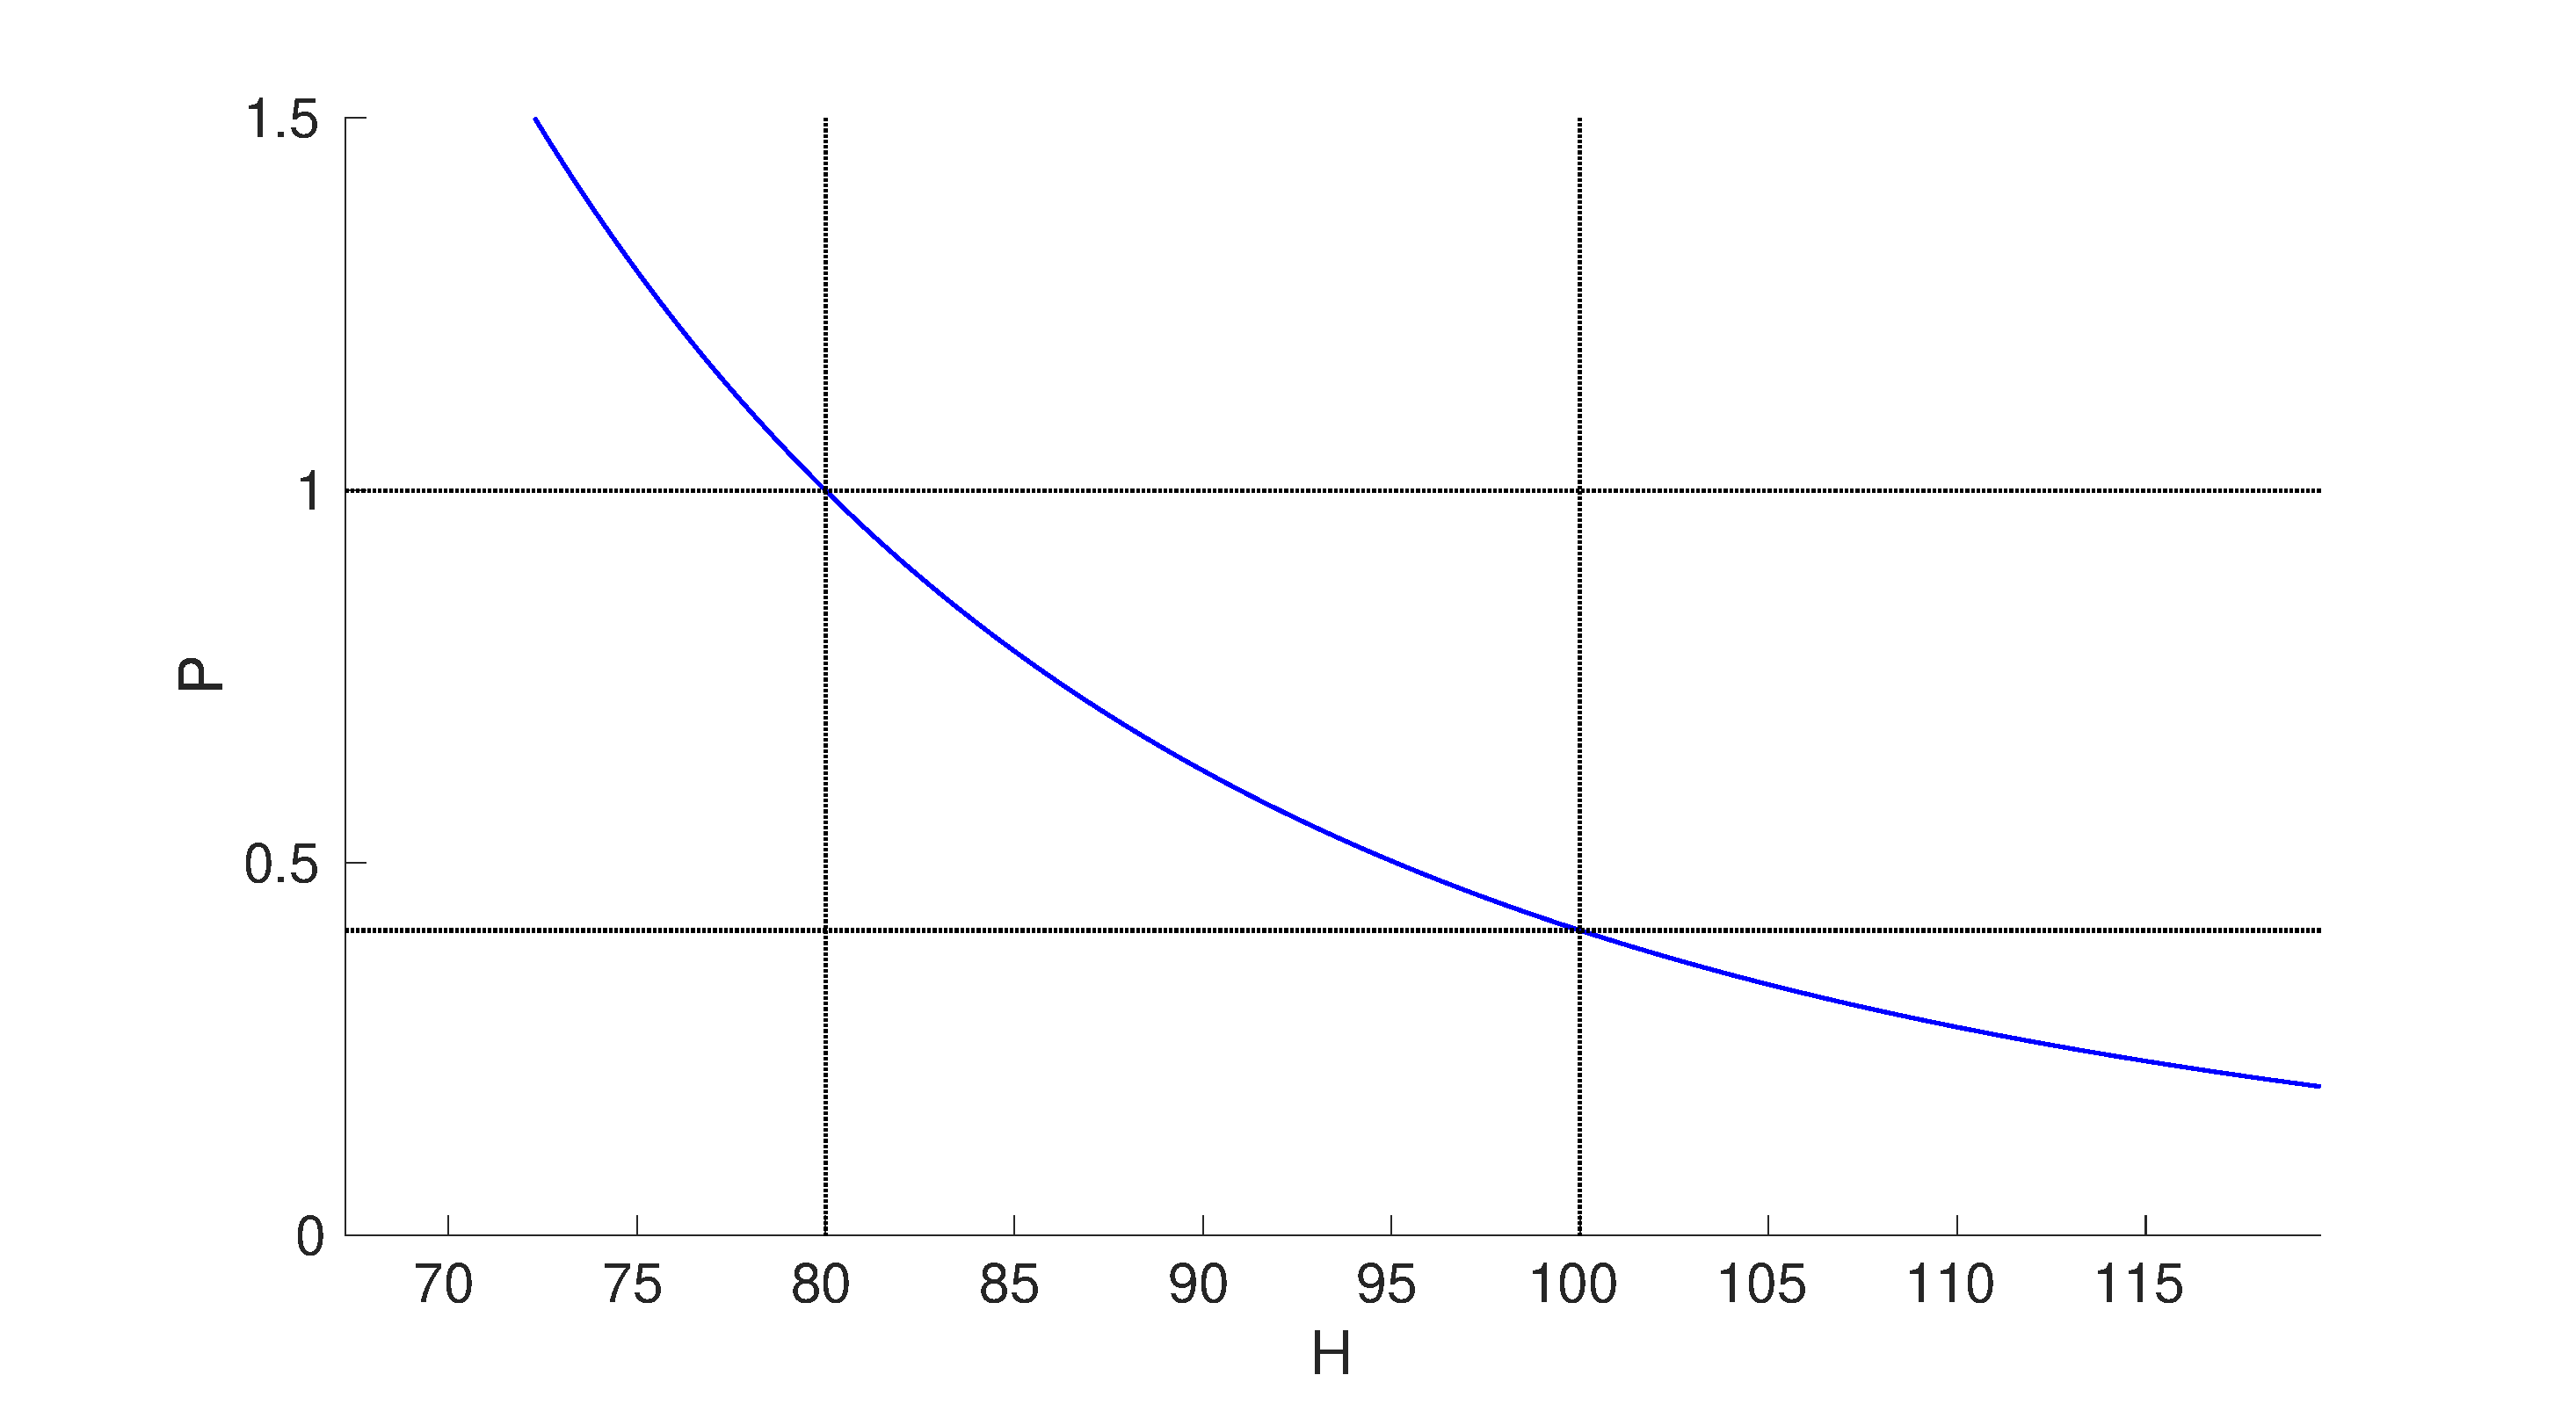
\includegraphics[width=12cm]{figure1.eps}\\
	\caption{Compensated demand curve for those whose optimal consumption on housing is $\$80$}\label{fig1}
\end{figure}

\begin{figure}[!htbp]
	\centering
	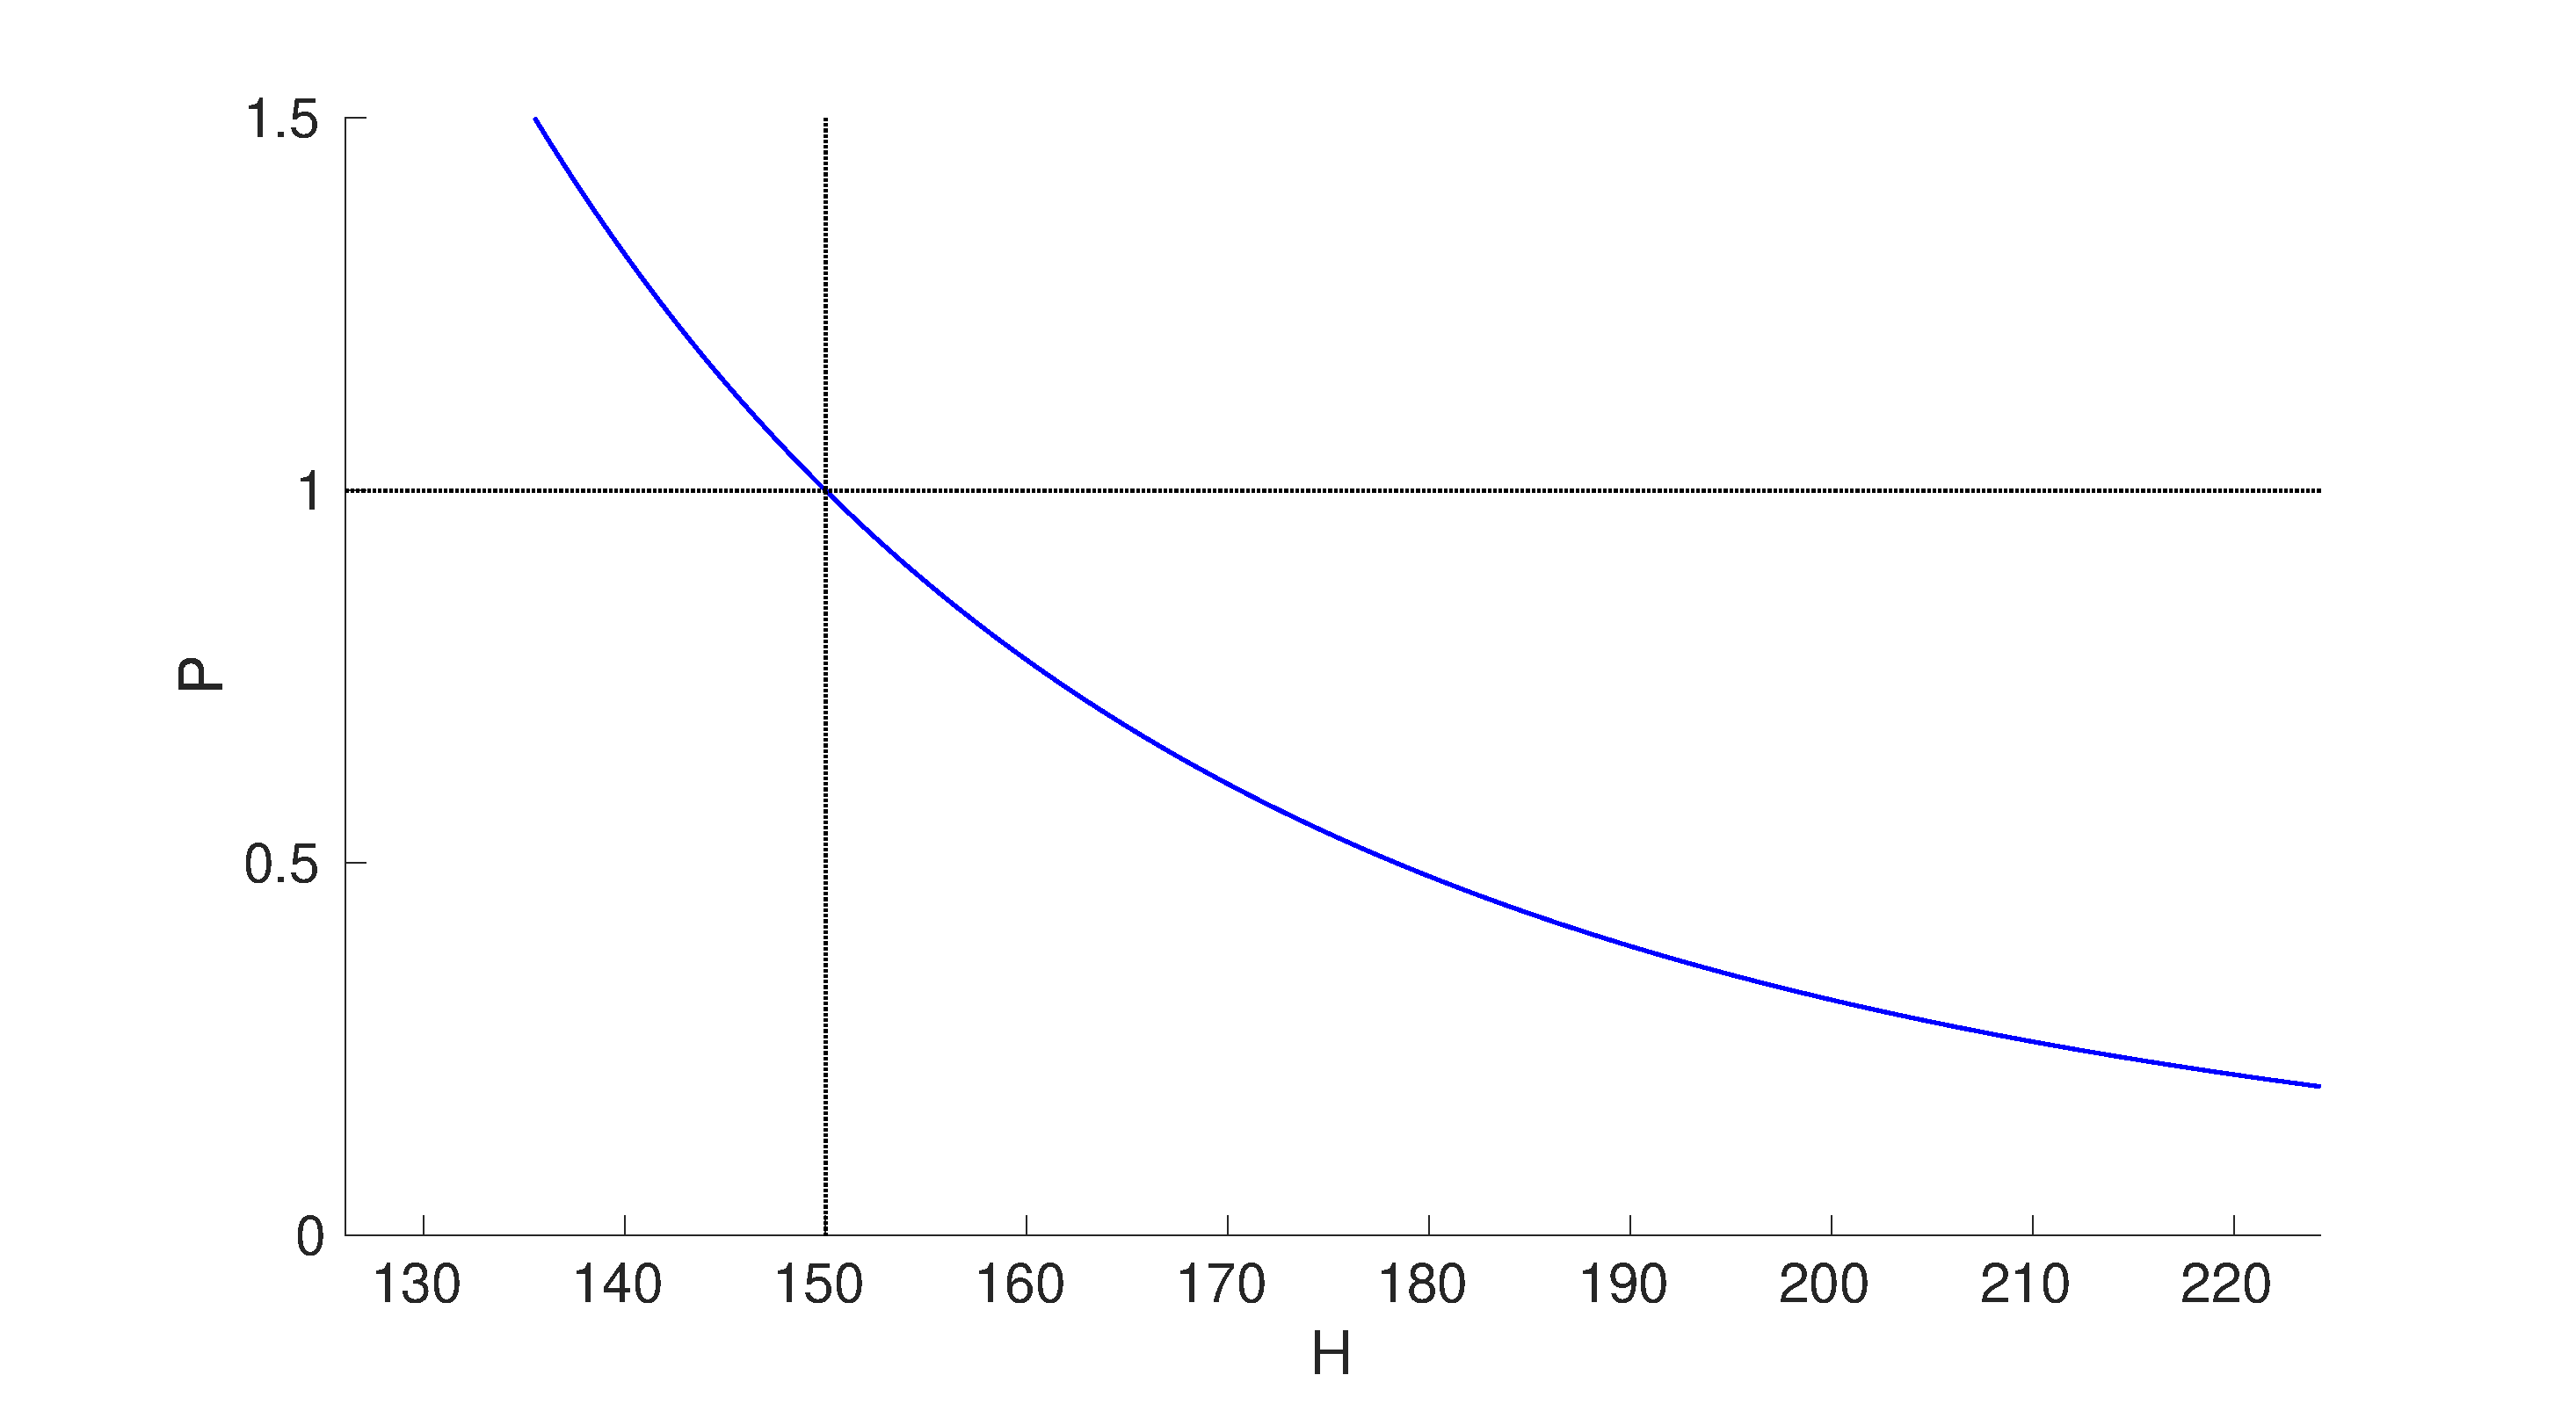
\includegraphics[width=12cm]{figure2.eps}\\
	\caption{Compensated demand curve for those whose optimal consumption on housing is $\$150$}\label{fig2}
\end{figure}

\subsubsection{Subpart (b)}
The estimation of deadweight loss is equivalent to estmation of the shaded area. This can be done by an integral.
\begin{align*}
	DWL&=\int_{80}^{100}(1-P(H))dH\\
	&=\int_{80}^{100}(H/80)^{-4}dH\\
	&\approx13.0
\end{align*}

Thus, the deadweight loss is approximately $\$13.0$ for those who are constrained. Since the constrained population is $50\%$ of the overall population, on average the deadweight loss is $\$6.5$ per person.

\subsection{Part (4)}
Compared with nothing, every recipient benefits. However, compared with receiving vouchers, those who originally spent $\$150$ on housing loses, since they were not constrained previously, and they receive less now. Those who originally did not spend additional money on housing benefits, since they receive more ($\$100-\$6.5=\$93.5$) than they would value the vouchers ($\$100-\$13.0=\$87.0$) under constraint.

\subsection{Part (5)}
No. Group 1 does not provide any number that is used in the calculation. It serves as a control group. It confirms the fact that half of the population are constrained.

\subsection{Part (6)}
No, I am NOT concerned. This is because the other $50\%$ people are unconstrained. As long as they spend more than $\$100$, they value the voucher as its full face value and do not contribute to DWL. So the previous calculation is unaffected.

\subsection{Part (7)}
\subsubsection{Subpart (a)}
When the constrained people value their vouchers below $\$0.75$, they will sell them. Their loss is reduced. Part of this loss ($25\%$ face value of the vouchers sold) should not be counted into the deadweight loss, for it goes to the criminals (middlemen who trade vouchers, or unconstrained people who want to buy more housing at a low price). This is, however, a loss in targeting efficiency, and it leads to a waste of public resources.

The total deadweight loss is the shaded area, which is smaller than before.
\begin{figure}[!htbp]
	\centering
	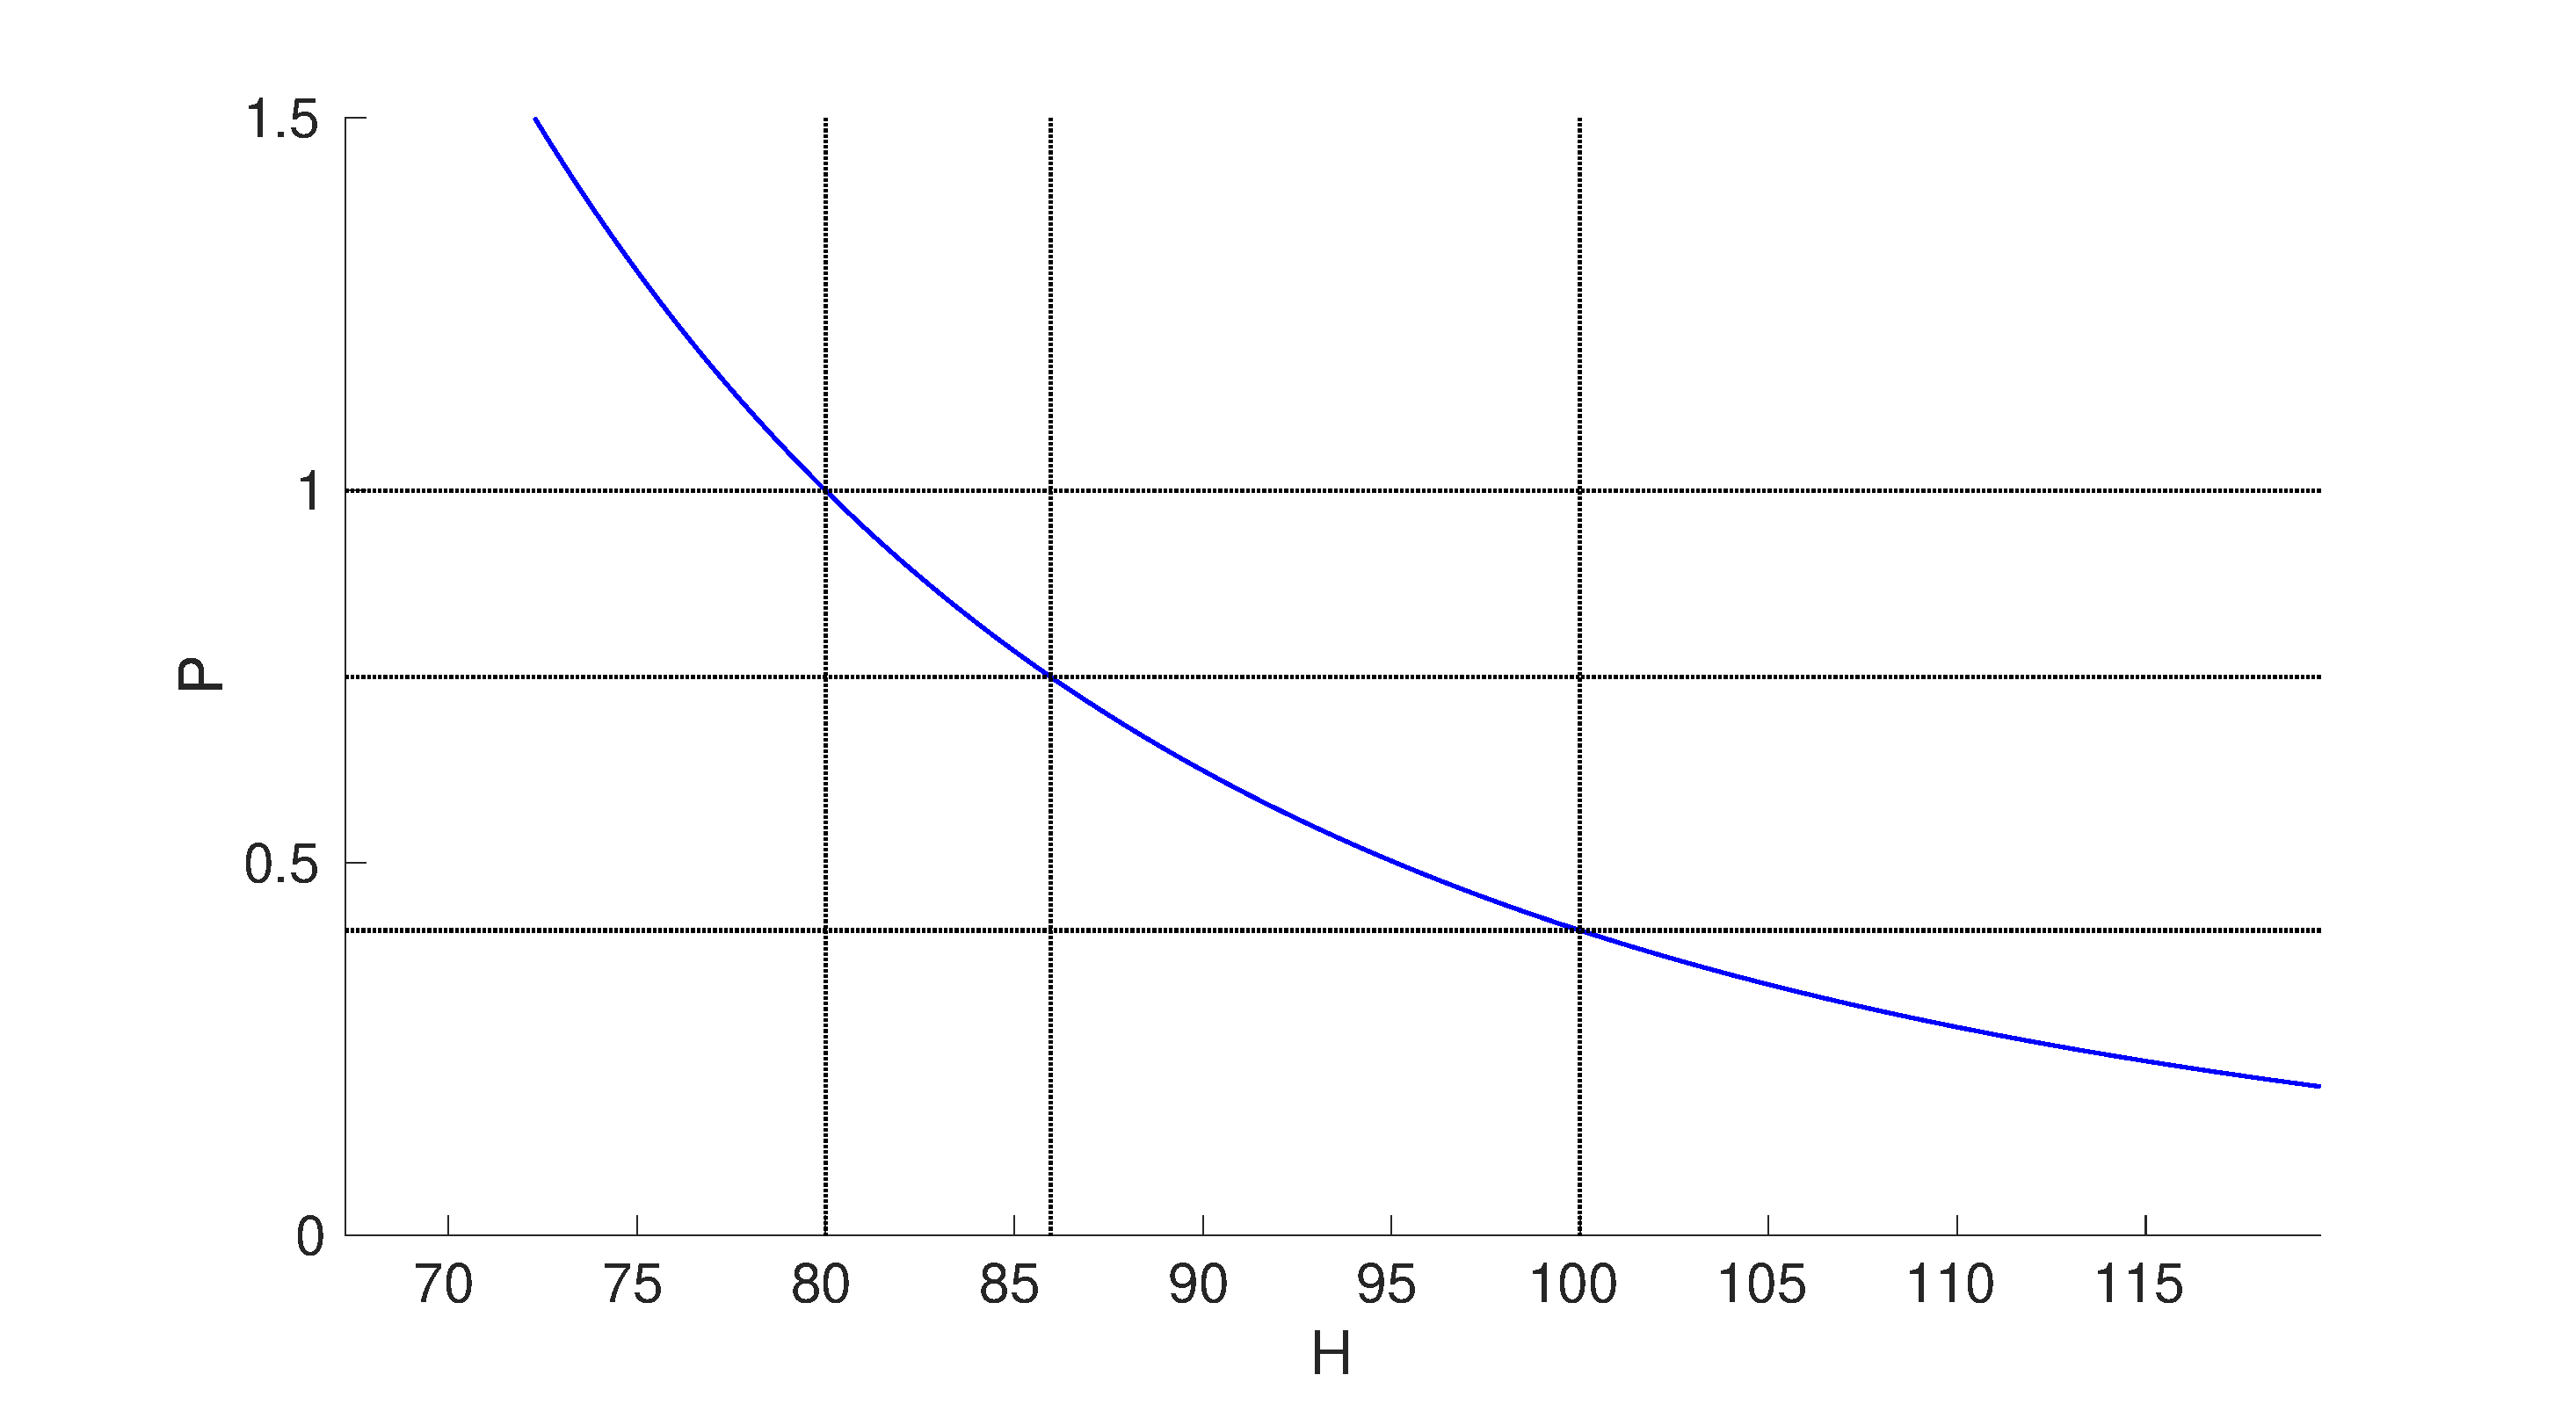
\includegraphics[width=12cm]{figure3.eps}
	\caption{Deadweight loss when there is a black market}\label{fig3}
\end{figure}

\subsubsection{Subpart (b)}
Yes, I will be concerned. If so, there should be something wrong in the model. Since even the constrained people value their vouchers no less than $(80/100)^4\approx41\%$ of their face value, it cannot be that someone wants to sell his/her $\$1$ voucher at $\$0.25$.

\end{document}
